\documentclass[10pt,a4paper]{article}
\usepackage[latin1]{inputenc}
\usepackage{amsmath}
\usepackage{float}
\usepackage{graphicx}
\usepackage{fullpage}
\usepackage{caption}
\usepackage{subfig}
\begin{document}
\captionsetup{width=0.8\textwidth}

\author{Jeroen Hofman\\
  University of Amsterdam \\
  		10194754\\
		}
\title{Stochastic Simulation Project 3\\
       Discrete event simulation: Elevator
		}
\maketitle

\newpage

\section{Introduction}
In this small report we simulate an elevator in a 4-floor building during morning rush hour. We look at the average travel time as a function of the arrival rate and we look at critical arrival rates, i.e. rates at which the queue in front of the elevator will keep growing. We study three different cases: all the people who arrive will join the queue, some people with the first floor as destination will not join the queue, and some people with any destination will not join the queue.

\section{Theory}
The elevator is simulated using a discrete event simulation. Discrete event simulations, in contrast to discrete time simulations, will only perform actions when an event takes place. By going from one event to another in chronological order the time parameter is updated every time.\\
\noindent In the case of the elevator simulation three different events have to be considered: 

\begin{itemize}
  \item
    The arrival of a person: Persons enter the simulation to possibly join the queue in front of the elevator. The arrival times are generated using a Poisson distribution, i.e. a distribution of the form:
    \begin{equation}
      f(k,\lambda) = \frac{\lambda^k e^\lambda}{k!}
    \end{equation}
    where $f(k,\lambda)$ is the probability density function as a function of $k$ occurrences in an interval with an average occurrence rate of $\lambda$ in that interval \cite{book}. In the elevator model $\lambda$ is equal to the mean time between arrivals, or MTBA for short. An arrival event can be scheduled by drawing randomly from this distribution.
  \item
    The departure of the elevator: As soon as a person arrives, a departure time is scheduled. The departure time is updated every time a new person arrives, details can be found in the section 'About the code'.
  \item
    The return of the elevator: If the elevator has departed, it will return after some time, depending on the amount of persons in the elevator and their destination, again details can be found in the section 'About the code'.
\end{itemize}

\noindent The arrival of a person triggers a departure event and a new arrival at some later time drawn from the Poisson distribution. A departure event triggers a return event, a return event triggers a new departure event. With a constant arrival of new persons this loop means that this system is self-sustaining.

\section{Methods}
In this model we compute the following parameters:

\begin{itemize}
  \item
    The queue time: When a person arrives, it possibly joins the queue in front of the elevator. The queue time is defined as the time between the arrival and the departure of the elevator containing that person. Hence having entered the elevator and waiting for departure of the elevator (when for instance other persons are still boarding) is also considered queue time for convenience.
  \item
    The travel time: The amount of time a person spends inside the elevator, beginning from the departure of the elevator, until the person has stepped out of the elevator.
\end{itemize}

\noindent The simulation starts with the scheduling of an arrival and then proceeds from one event to the next, described in the previous section. The simulation is run for a fixed time $T_{\text{max}}$ and measurements on the above two quantities are performed on evenly spaced intervals in this time span. After every such a measurement interval the average queuing time and the average travel time are computed, and they are summed up in the average journey time for a person in that interval. By taking the average over all these intervals of the average journey time, a final estimate with an error is obtained for the average journey time (strictly speaking the average of the average journey time).
It has to be taken into account that if the MTBA is too low, the queue will grow over time, because the elevator cannot keep up with the number of persons that arrive and join the queue. In this case it is not useful to compute the average journey time, since it will grow from one measurement interval to the next and hence the final estimate for the average journey time will not be accurate and fully dependent on $T_{\text{max}}$ and the measurement intervals. To avoid this the difference between the average journey time over two subsequent measurement intervals is computed. The mean difference with corresponding error is computed over all pairs of subsequent measurement intervals. If this mean difference is close to zero, it means that subsequent measurements intervals will give roughly the same mean and so the queue is not growing over time.\\
\newline
When a person arrives, it can be given a choice whether or not to join the queue. In this report we investigate the following three scenarios:

\begin{enumerate}
  \item
    All persons that arrive according to the Poisson distribution join the queue, regardless of their destination.
  \item
    When a person arrives and has its destination set to the first floor, it has a probability of not joining the queue, i.e. taking the stairs, given by $1 - c^{|q|}$, where $0 < c < 1$ is some parameter and $|q|$ is the length of the queue.
  \item
    When a person arrives and has destination $dest$, with $1 \leq dest \leq 4$, it has a probability of joining the queue given by $1 - \frac{c^{|q|}}{dest}$
\end{enumerate}

\noindent The expectation is that the average queue length will decrease for scenarios (2) and (3).

\section{Results}

We run the simulation with $T_{\text{max}} = 10^6$, measuring for 1000 time steps every 2000 time steps (so measurements are made for $1000 < t \leq 2000$, $3000 < t \leq < 4000$ etc.). We calculated the average journey time from these time intervals, as described in the previous section, for the three different scenarios with $c = 0.9$ and for $5 \leq \text{MTBA} \leq 34$. The figure below shows the average difference between measurements on two subsequent time intervals for all the three scenarios, as a function of the mean time between arrivals. If the measurements are uncorrelated this should give zero, indicating that the queue is not growing between subsequent measurement intervals, and hence that the elevator can keep up with the arrival rate of persons. For case (1) it is seen that the minimum MTBA is $\geq 14$, for case (2) it is MTBA $\geq 9$ and for case (3) MTBA $\geq 6$. Clearly the effect of persons not joining the queue is visible here, since in case (2) and (3) the MTBA can be lower and still have a queue which does not explode.

\begin{figure}[H]
  \centering
  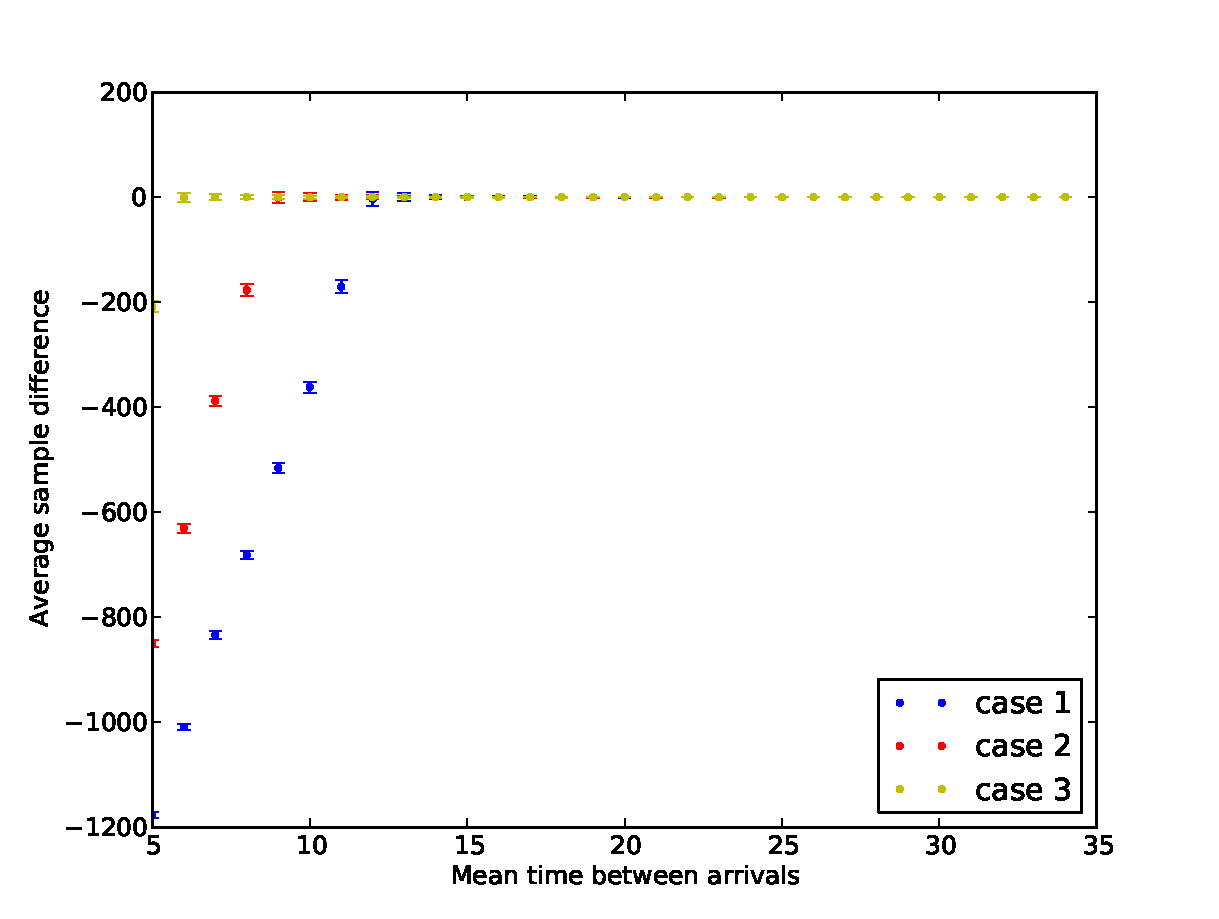
\includegraphics[width=0.7\textwidth]{diff.pdf}
  \caption{The average difference between two subsequent measurement intervals as a function of the MTBA for the three different cases. The error bars correspond to a 5\% confidence interval.}
  \label{fig:diff}
\end{figure}

\noindent Figure \ref{fig:journey} below shows the average journey time for the three cases as a function of the MTBA, shown only for MTBA values greater than the minimum value found in the previous paragraph in order to make a fair comparison. We see that all three curves follow an exponential or power law decay in the average journey time as a function of the MTBA. Also the difference for low MTBA between the cases is significant, but decreases rapidly for increasing MTBA. This is expected since when the MTBA increases all cases should converge to the same journey time, namely the time it takes for one person to arrive, depart with the elevator and disembark at its location, since the next arrival will not take place before the departure of the elevator when the MTBA is very large. The person will also never take the stairs, because the length of the queue is zero for these large values of the MTBA.

\begin{figure}[H]
  \subfloat{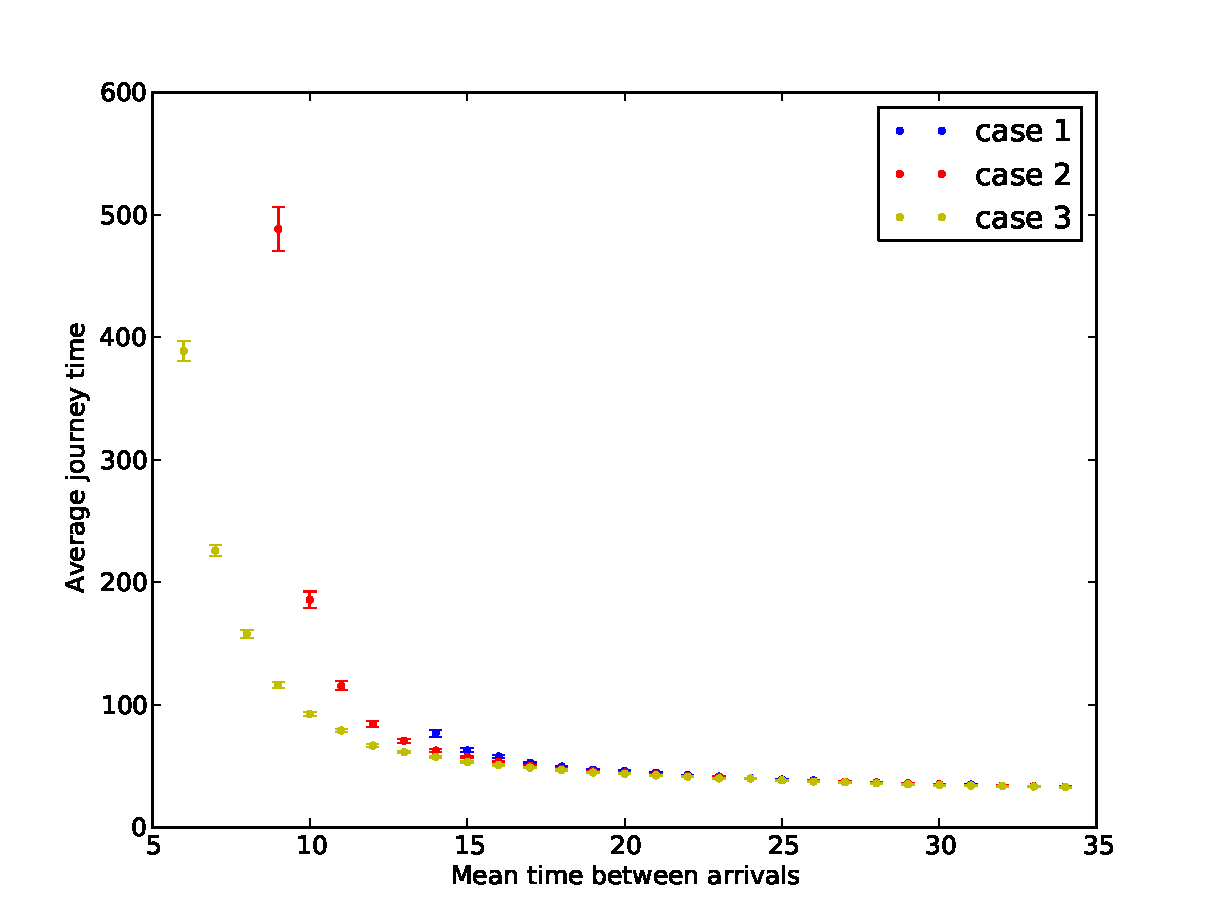
\includegraphics[width=0.5\textwidth]{journey1.pdf}}
  \subfloat{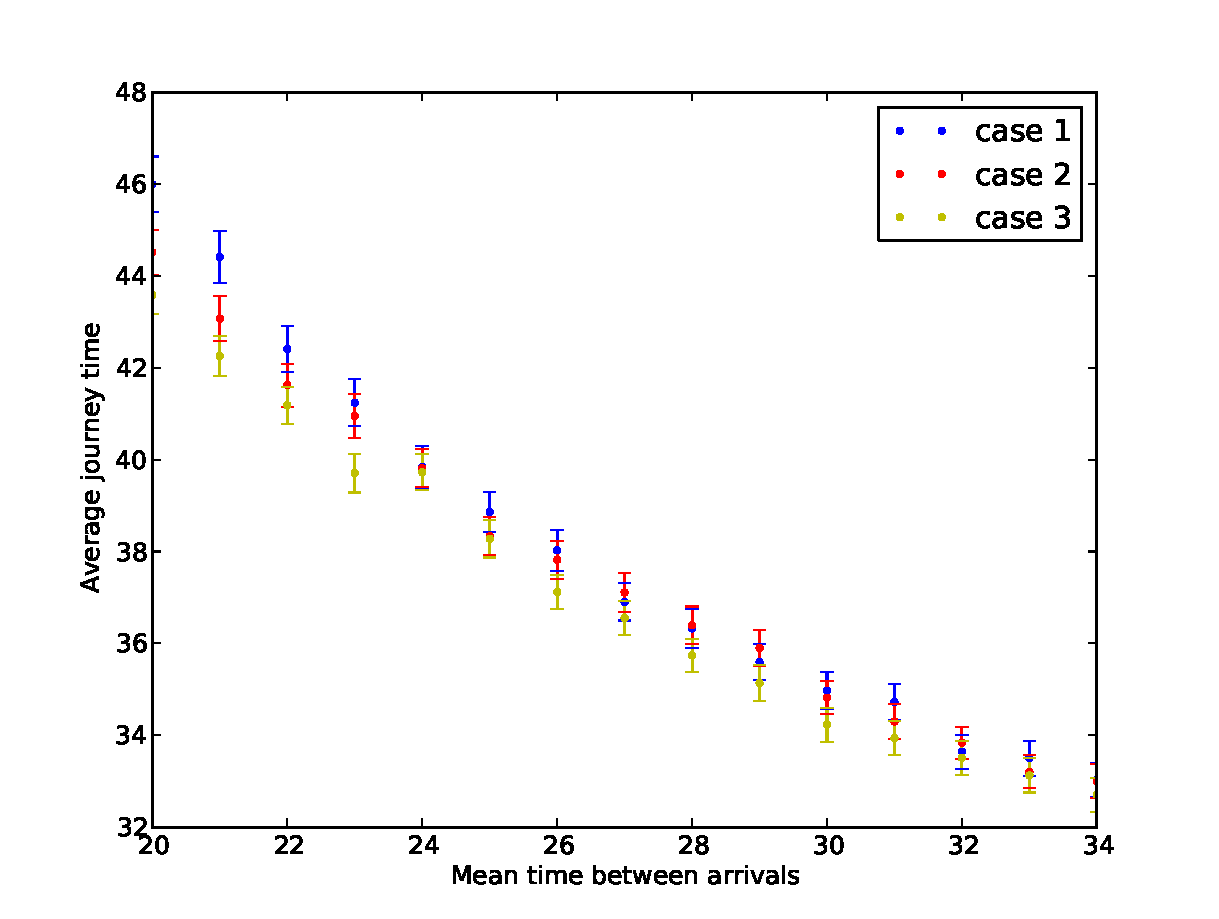
\includegraphics[width=0.5\textwidth]{journey2.pdf}}
  \caption{The average journey time as a function of the MTBA for all three cases. The left figure shows all the allowed values, excluding the values for which the queue explodes over time. The right figure zooms in on the right part of the left figure to show the convergence. The error bars correspond to a 5\% confidence interval.}
  \label{fig:journey}
\end{figure}

\section{Discussion}

In this report we considered a discrete event simulation of an elevator in the morning rush hour. A first thing to note is that the elevator is not capable of handling a MTBA below 14 in case (1) which, in terms of seconds, can be the case in the morning rush hour. It makes a significant difference however whether or not persons are allowed to take the stairs, which is a more realistic case (also judging from my own experience).\\
The average travel time for the elevator is around 80 seconds for case (1) (this can be calculated from the parameters), this also gives a lower bound for the MTBA, given by 80/6 = 13.3, assuming the capacity of the elevator is six people. So indeed the minimum MTBA found by the simulation is close to the theoretical minimum, given by 13.3.\\
If we assume that the average journey time decreases exponentially with increasing MTBA, it will have an asymptote. Using the values from the model (see 'About the code') we can actually calculate this asymptote by taking a very large MTBA, such that one person arrives, gets in the elevator and gets out of the elevator and the elevator returns before the next person arrives. The average travel time should be 19.5 with the current parameters in the model.
\newline
\noindent Improvements for the model might be to look at multiple elevators, but since I wrote my program not in an object-oriented way, this was too much work to implement within the current time frame. Also one might consider different formulas for the probability of queuing or taking the stairs, the formulas used in this report are just simple rules, which I thought of having some validity. Of course another thing to implement is to let people also take the elevator from higher floors down or up, so as to be able to model the elevator also during other times of the day. In the case of multiple elevators you might want to create an intelligent system, which communicates and is self-learning in this case. This is however well beyond of the scope of this project.

\section{About the code}

I have written the simulation in Python, because of its easy handling of arrays and queue objects. I decided not to write my program object oriented, because it is not really necessary in this case. Instead I use three different functions which schedule the arrival event, the departure event and the return event. There is a loop over the MTBA and every such case starts with a single arrival event, this arrival event triggers a departure event, which is updated if other persons arrive before the elevator leaves. When the elevator leaves persons still keep arriving but automatically join the queue and they do not update the departure time anymore. Whenever the elevator departs, it sets a return time, which is a function of the number of people in the elevator and their destinations. There are different constants for opening the elevator door, closing the elevator door, entering/leaving the elevator for a single person, the acceleration/deceleration of the elevator and the time between subsequent floors at full speed. The constants are based upon my own experience with elevators and also some wild guesses. For a fully loaded elevator, which has a capacity of six persons in my simulation, the average time to return is about 80 seconds, which seemed reasonable to me. I realize the function that schedules the return event can be written much more efficiently, i.e. just one or two lines computing the return time of the elevator as a function of the persons in the elevator and their destinations, however for the sake of being able to keep track of what is happening I wrote the code person by person and in this format it was easy to determine the time when people get out of the elevator, while in the one or two line code you have to do that separately.
In the code I use special queue objects from the class collections, which is a standard python class. It provides very fast pop and append operations. I have to convert it once in the return function to a list because these objects cannot be sorted. 

\begin{thebibliography}{15}
\bibitem{book}
  Ross, S.M., \emph{Simulation}, 2006, Academic Press
\end{thebibliography}

\end{document}